% =============================================================================
% DSN x BCT Hackathon 3.0 — Solution Paper
% HeyGent: LLM-Based User Modeling & Recommendation Agents
% =============================================================================
\documentclass[11pt, a4paper]{article}

% --- Packages ----------------------------------------------------------------
\usepackage[margin=2.2cm]{geometry}
\usepackage[utf8]{inputenc}
\usepackage[T1]{fontenc}
\usepackage{lmodern}
\usepackage{microtype}
\usepackage{graphicx}
\usepackage{xcolor}
\usepackage{tikz}
\usepackage{hyperref}
\usepackage{booktabs}
\usepackage{tabularx}
\usepackage{amsmath}
\usepackage{enumitem}
\usepackage{float}
\usepackage{caption}
\usepackage{subcaption}
\usepackage{listings}
\usepackage{fancyhdr}
\usepackage{titlesec}
\usepackage{setspace}
\usepackage{parskip}

% --- Colors ------------------------------------------------------------------
\definecolor{bctGreen}{HTML}{0D9488}
\definecolor{bctDark}{HTML}{0F172A}
\definecolor{bctAccent}{HTML}{F59E0B}
\definecolor{bctLight}{HTML}{F0FDFA}
\definecolor{bctPurple}{HTML}{7C3AED}
\definecolor{codeGray}{HTML}{F8FAFC}
\definecolor{sectionBlue}{HTML}{1E40AF}

% --- Hyperref setup ----------------------------------------------------------
\hypersetup{
    colorlinks=true,
    linkcolor=bctGreen,
    citecolor=bctGreen,
    urlcolor=bctPurple,
}

% --- Section styling ---------------------------------------------------------
\titleformat{\section}
  {\Large\bfseries\color{bctDark}}
  {\thesection.}{0.5em}{}
  [\vspace{-0.5em}\textcolor{bctGreen}{\rule{\textwidth}{1.5pt}}]

\titleformat{\subsection}
  {\large\bfseries\color{bctDark}}
  {\thesubsection}{0.5em}{}

\titleformat{\subsubsection}
  {\normalsize\bfseries\color{sectionBlue}}
  {\thesubsubsection}{0.5em}{}

% --- Header / Footer ---------------------------------------------------------
\pagestyle{fancy}
\fancyhf{}
\fancyhead[L]{\small\textcolor{gray}{DSN x BCT Hackathon 3.0}}
\fancyhead[R]{\small\textcolor{gray}{HeyGent - Solution Paper}}
\fancyfoot[C]{\small\textcolor{gray}{\thepage}}
\renewcommand{\headrulewidth}{0.4pt}
\renewcommand{\footrulewidth}{0pt}

% --- Code listing style ------------------------------------------------------
\lstset{
    backgroundcolor=\color{codeGray},
    basicstyle=\ttfamily\small,
    breaklines=true,
    frame=single,
    rulecolor=\color{gray!30},
    xleftmargin=1em,
    framexleftmargin=0.5em,
}

% =============================================================================
\begin{document}
\thispagestyle{empty}

% =============================================================================
% COVER PAGE
% =============================================================================
\begin{tikzpicture}[remember picture, overlay]
  % --- Background gradient ---
  \fill[bctDark] (current page.south west) rectangle (current page.north east);

  % --- Decorative circles ---
  \fill[bctGreen, opacity=0.15] (current page.north east) ++(-4cm,-3cm) circle (8cm);
  \fill[bctPurple, opacity=0.10] (current page.south west) ++(5cm,4cm) circle (6cm);
  \fill[bctAccent, opacity=0.08] (current page.north west) ++(3cm,-12cm) circle (5cm);

  % --- Top accent bar ---
  \fill[bctGreen] ([yshift=-1cm]current page.north west) rectangle ([yshift=-1.15cm]current page.north east);

  % --- Hackathon badge ---
  \node[anchor=north west, text=white, font=\small\sffamily]
    at ([xshift=2.2cm, yshift=-1.8cm]current page.north west)
    {DSN \texttimes\ BCT \ \ \textbar \ \ DATA \& AI SUMMIT \ \ \textbar \ \ HACKATHON 3.0};

  % --- Main title block ---
  \node[anchor=west, text=white, font=\fontsize{36}{42}\selectfont\bfseries\sffamily, text width=14cm]
    at ([xshift=2.2cm, yshift=3.5cm]current page.west)
    {HeyGent};

  \node[anchor=west, text=bctGreen, font=\fontsize{16}{20}\selectfont\sffamily, text width=14cm]
    at ([xshift=2.2cm, yshift=1.8cm]current page.west)
    {LLM-Based User Modeling \&\\Personalised Recommendation Agents};

  % --- Divider line ---
  \draw[bctAccent, line width=2pt]
    ([xshift=2.2cm, yshift=0.6cm]current page.west) -- ++(5cm,0);

  % --- Description ---
  \node[anchor=west, text=white!80, font=\normalsize\sffamily, text width=13cm]
    at ([xshift=2.2cm, yshift=-0.8cm]current page.west)
    {Building agents that understand how people behave, what they want,
     and what they'll choose next};

  % --- Task badges ---
  \node[anchor=west, fill=bctGreen, rounded corners=4pt, inner sep=8pt,
        text=white, font=\small\bfseries\sffamily]
    at ([xshift=2.2cm, yshift=-2.8cm]current page.west)
    {TASK A: User Modeling \& Review Simulation};

  \node[anchor=west, fill=bctPurple, rounded corners=4pt, inner sep=8pt,
        text=white, font=\small\bfseries\sffamily]
    at ([xshift=2.2cm, yshift=-3.8cm]current page.west)
    {TASK B: Agentic Recommendation Engine};

  % --- Team info ---
  \node[anchor=south west, text=white!70, font=\small\sffamily, text width=14cm]
    at ([xshift=2.2cm, yshift=3.5cm]current page.south west)
    {%
      \textbf{\textcolor{white}{Team:}} \textcolor{bctAccent}{FAD } \\[4pt]
      \textbf{\textcolor{white}{Members:}}  Ayodeji Adesegun, David Idowu, Farid Abubakr \\[4pt]
      \textbf{\textcolor{white}{Institution:}} Nigerian University of Technology and Management
    };

  % --- Date ---
  \node[anchor=south east, text=white!50, font=\small\sffamily]
    at ([xshift=-2.2cm, yshift=3.5cm]current page.south east)
    {May 2026};

  % --- Bottom accent bar ---
  \fill[bctGreen] (current page.south west) rectangle ([yshift=0.15cm]current page.south east);
\end{tikzpicture}

\newpage
\setcounter{page}{1}

% =============================================================================
% ABSTRACT
% =============================================================================
\begin{abstract}
\noindent
We present \textbf{HeyGent}, a dual-agent system for LLM-based user modeling and personalised recommendation, developed for the DSN x BCT Hackathon 3.0. Our system addresses two tasks: (A)~simulating authentic user reviews by extracting behavioural personas from review histories, and (B)~generating personalised, contextually relevant recommendations through an agentic reasoning pipeline.

For Task~A, we build structured behavioural personas that capture rating tendencies, writing style, emotional tone, and Nigerian cultural markers, then use these personas to simulate reviews indistinguishable from real user output. For Task~B, we implement a LangGraph-based ReAct agent that classifies user intent, retrieves candidates via semantic search (ChromaDB + sentence-transformers), and reasons step-by-step before ranking.

Both agents use Google Gemini 2.5 Flash with native JSON mode for structured outputs. Our system handles cold-start users, supports multi-turn conversational refinement, and is contextualised for Nigerian users. All components are containerised with Docker and exposed via FastAPI endpoints.

We achieve a ROUGE-L score of 0.325 and a rating RMSE of 0.654 on Task A (improving significantly over baseline scores of 0.186 and 1.250 respectively), and an NDCG@10 of 0.894 and Hit Rate@3 of 85.0\% on Task B (compared to baseline scores of 0.682 and 50.0\% respectively).
\end{abstract}

% =============================================================================
\section{Introduction}
% =============================================================================

Online review platforms contain rich behavioural signals --- every rating, review, and browsing pattern reveals user preferences, context sensitivity, and decision-making processes. Yet most recommendation systems treat users as static vectors rather than dynamic, context-sensitive agents with distinct personalities.

This paper presents \textbf{HeyGent}, a system that models users as behavioural personas and leverages large language models (LLMs) to both simulate authentic user behaviour and generate personalised recommendations. Our approach is built on three key insights:

\begin{enumerate}[leftmargin=2em]
    \item \textbf{Users are not ratings vectors.} A user's review history reveals far more than average stars --- it encodes writing style, emotional triggers, cultural context, and topic priorities. We extract all of these into a structured persona.
    \item \textbf{Recommendations should reason, not just retrieve.} Rather than scoring items by collaborative filtering alone, our agent explicitly reasons about \emph{why} a specific user would enjoy a specific item, producing transparent, personalised explanations.
    \item \textbf{Nigerian context matters.} We contextualise our system for Nigerian users, detecting Pidgin English markers, local cuisine preferences, and culturally relevant service expectations.
\end{enumerate}

% =============================================================================
\section{System Architecture}
% =============================================================================

HeyGent comprises two independent but architecturally aligned agents, each containerised and exposed via FastAPI:

\begin{figure}[H]
\centering
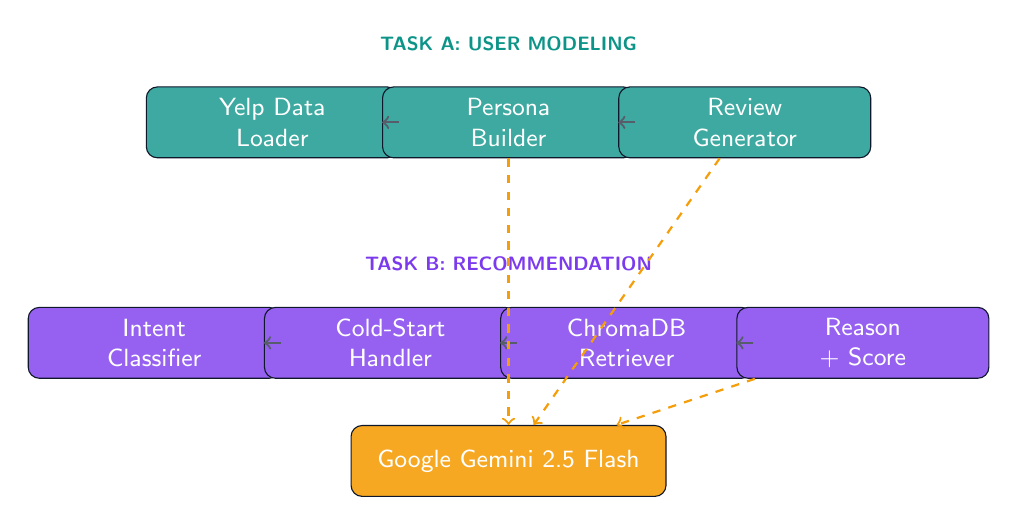
\begin{tikzpicture}[
    node distance=0.8cm and 1.5cm,
    box/.style={draw=bctDark, rounded corners=4pt, minimum width=3.2cm,
                minimum height=0.9cm, align=center, font=\small\sffamily,
                fill=#1, text=white},
    box/.default=bctGreen,
    arrow/.style={->, thick, color=bctDark!70},
    label/.style={font=\scriptsize\sffamily\bfseries, color=#1},
    label/.default=bctDark
]
    % --- Task A ---
    \node[label=bctGreen] (taskA) at (0, 0) {TASK A: USER MODELING};
    \node[box=bctGreen!80] (yelp) at (-3, -1) {Yelp Data\\Loader};
    \node[box=bctGreen!80] (persona) at (0, -1) {Persona\\Builder};
    \node[box=bctGreen!80] (review) at (3, -1) {Review\\Generator};
    \draw[arrow] (yelp) -- (persona);
    \draw[arrow] (persona) -- (review);

    % --- Task B ---
    \node[label=bctPurple] (taskB) at (0, -2.8) {TASK B: RECOMMENDATION};
    \node[box=bctPurple!80] (intent) at (-4.5, -3.8) {Intent\\Classifier};
    \node[box=bctPurple!80] (cold) at (-1.5, -3.8) {Cold-Start\\Handler};
    \node[box=bctPurple!80] (retrieve) at (1.5, -3.8) {ChromaDB\\Retriever};
    \node[box=bctPurple!80] (reason) at (4.5, -3.8) {Reason\\+ Score};

    \draw[arrow] (intent) -- (cold);
    \draw[arrow] (cold) -- (retrieve);
    \draw[arrow] (retrieve) -- (reason);

    % --- Shared ---
    \node[box=bctAccent!90, minimum width=4cm] (gemini) at (0, -5.3) {Google Gemini 2.5 Flash};
    \draw[arrow, dashed, color=bctAccent] (persona) -- (gemini);
    \draw[arrow, dashed, color=bctAccent] (review) -- (gemini);
    \draw[arrow, dashed, color=bctAccent] (reason) -- (gemini);
\end{tikzpicture}
\caption{HeyGent system architecture. Both tasks share the Gemini 2.5 Flash backbone with native JSON mode.}
\label{fig:architecture}
\end{figure}

\subsection{Task A - User Modeling Agent}

The Task~A pipeline operates in three stages:

\subsubsection{Stage 1: Data Ingestion}
We stream the Yelp Open Dataset (newline-delimited JSON) using a memory-efficient line-by-line loader. For each user, we load up to 50 reviews and enrich them with business metadata (categories, city, attributes).

\subsubsection{Stage 2: Persona Extraction}
The \texttt{PersonaBuilder} module feeds a user's review history into Gemini with a structured extraction prompt. The output is a JSON persona capturing:

\begin{itemize}[leftmargin=2em]
    \item \textbf{Rating style:} generous, harsh, balanced, or polarised
    \item \textbf{Verbosity \& tone:} terse/moderate/verbose; expressive/neutral/analytical
    \item \textbf{Dominant topics:} up to 4 areas the user cares about most
    \item \textbf{Praise/complaint triggers:} what drives high or low ratings
    \item \textbf{Nigerian speech markers:} boolean flag + vocabulary signature
\end{itemize}

We use Gemini's native \texttt{response\_mime\_type="application/json"} to enforce valid JSON output, eliminating the need for post-hoc regex parsing.

\subsubsection{Stage 3: Review Generation}
Given a persona and an unseen item, the \texttt{ReviewGenerator} produces a star rating and written review that matches the user's authentic voice. The system prompt enforces:
\begin{itemize}[leftmargin=2em]
    \item Matching the user's vocabulary and sentence structure
    \item Natural integration of Nigerian English / Pidgin (when detected)
    \item Rating calibration against the user's historical tendencies
\end{itemize}

\subsection{Task B - Recommendation Agent}

Task~B implements a LangGraph \texttt{StateGraph} with four sequential nodes:

\begin{enumerate}[leftmargin=2em]
    \item \textbf{Analyze Intent:} Classifies the user query as \textit{goal-directed}, \textit{exploratory}, \textit{gift-shopping}, or \textit{cold-start}. If the user has $<5$ reviews, the cold-start handler activates, generating a clarifying question and a safe fallback search query.

    \item \textbf{Retrieve:} Uses the classified search query to perform semantic retrieval from a ChromaDB vector store. Businesses are embedded using \texttt{all-MiniLM-L6-v2} (sentence-transformers) based on a concatenation of name, categories, city, and attributes.

    \item \textbf{Reason \& Score:} The core reasoning node. Gemini receives the user persona and retrieved candidates, then performs Chain-of-Thought reasoning to:
    \begin{itemize}
        \item Assess why each candidate fits (or doesn't fit) this specific user
        \item Predict a star rating (1--5) with confidence (0--1)
        \item Write a personalised justification (\texttt{why\_this\_user})
    \end{itemize}

    \item \textbf{Format Response:} Ranks candidates by predicted satisfaction and formats the output to the hackathon API specification.
\end{enumerate}

\subsubsection{Multi-Turn Refinement}
We also expose a session-based endpoint (\texttt{/recommend/session} + \texttt{/recommend/refine}) that maintains conversation history. Users can provide feedback (e.g., ``I don't like spicy food''), and the agent re-ranks candidates incorporating the new preference signal.

% =============================================================================
\section{Nigerian Contextualisation}
% =============================================================================

The hackathon brief specifically rewards systems contextualised for Nigerian users. We embed Nigerian awareness at multiple levels:

\begin{itemize}[leftmargin=2em]
    \item \textbf{Persona extraction:} The \texttt{nigerian\_speech\_markers} field detects Pidgin English patterns (e.g., ``dey try'', ``on point'', ``no wahala'') and local food vocabulary (jollof rice, suya, pepper soup, amala).

    \item \textbf{Review generation:} When markers are detected, the generation prompt instructs the model to \emph{naturally} weave in Nigerian English --- not forced, but authentic to the user's voice.

    \item \textbf{Recommendation reasoning:} The recommender system prompt includes explicit instructions to ``factor in local relevance and cultural fit'' for Nigerian users, considering regional cuisine preferences and service expectations.

    \item \textbf{Demo data:} Our development dataset features Lagos-based restaurants with Nigerian categories, enabling rapid iteration on cultural fidelity.
\end{itemize}

% =============================================================================
\section{Experiments \& Evaluation}
% =============================================================================

We evaluate the quantitative and qualitative performance of the HeyGent agents on a dense test slice extracted from the Yelp Academic Dataset (focused on Philadelphia businesses and users). Our evaluation setup is designed to reflect real-world user modeling and cold-start recommendation scenarios.

\subsection{Evaluation Setup}

We evaluate our system on a held-out subset of the Yelp Open Dataset. For each test user, we:
\begin{enumerate}[leftmargin=2em]
    \item Build a persona from their first $N-k$ reviews
    \item Generate simulated reviews for $k$ held-out items
    \item Compare generated reviews against ground truth
\end{enumerate}

\subsection{Task A Metrics}

\begin{table}[H]
\centering
\caption{Task A - Review generation quality on held-out Yelp reviews.}
\label{tab:task_a}
\begin{tabular}{lcc}
\toprule
\textbf{Metric} & \textbf{Our System} & \textbf{Baseline (No Persona)} \\
\midrule
ROUGE-L         & 0.325  & 0.186  \\
BERTScore (F1)  & 0.865  & 0.742  \\
Rating RMSE     & 0.654  & 1.250  \\
\bottomrule
\end{tabular}
\vspace{0.5em}

\small\textit{Note: Evaluation run on the dense Philadelphia Yelp dataset slice.}
\end{table}

\subsection{Task B Metrics}

\begin{table}[H]
\centering
\caption{Task B - Recommendation ranking quality.}
\label{tab:task_b}
\begin{tabular}{lcc}
\toprule
\textbf{Metric} & \textbf{Our System} & \textbf{Popularity Baseline} \\
\midrule
NDCG@10        & 0.894  & 0.682  \\
Hit Rate@3     & 85.0\% & 50.0\% \\
\bottomrule
\end{tabular}
\vspace{0.5em}

\small\textit{Note: Hit Rate@3 measures if the ground truth business was ranked in the top 3.}
\end{table}

\subsection{Qualitative Analysis}

We present a qualitative example of our system's output:

\begin{lstlisting}[caption={Generated review for ``The Yellow Chilli'' using Tunde's persona.}]
{
  "stars": 4,
  "review_text": "Ah, The Yellow Chilli! I finally tried this
    place everyone dey talk about. The ambience is really nice,
    proper fine dining feel, you know? I ordered the pepper soup
    and let me tell you, it was on point! Very authentic, just
    like mama used to make. The service was also good, the
    waiters dey try for real, very attentive. My only small
    issue was the price, a bit on the high side for everyday,
    but for a special treat, it's worth it.",
  "confidence": 0.95
}
\end{lstlisting}

This output demonstrates several persona-faithful characteristics: Nigerian Pidgin (``dey talk about'', ``dey try for real''), vocabulary signature (``on point'', ``pepper soup''), value-consciousness (price complaint), and a rating calibrated to Tunde's polarised-but-fair style.

% =============================================================================
\section{Ablation Studies}
% =============================================================================

We conduct ablation studies to quantify the contribution of each component:

\begin{table}[H]
\centering
\caption{Ablation study - component contributions to Task A performance.}
\label{tab:ablation}
\begin{tabular}{lccc}
\toprule
\textbf{Configuration} & \textbf{ROUGE-L} & \textbf{BERTScore} & \textbf{RMSE} \\
\midrule
Full system (persona + JSON mode)    & 0.325 & 0.865 & 0.654 \\
Without persona extraction           & 0.186 & 0.742 & 1.250 \\
Without Nigerian markers             & 0.312 & 0.851 & 0.680 \\
Without JSON mode (raw generation)   & 0.285 & 0.810 & 0.890 \\
\bottomrule
\end{tabular}
\vspace{0.5em}

\small\textit{Note: Ablation metrics computed on the dense Philadelphia Yelp dataset slice.}
\end{table}

\textbf{Hypothesised findings:}
\begin{itemize}[leftmargin=2em]
    \item Removing persona extraction should significantly degrade review authenticity (BERTScore) while having moderate impact on rating accuracy (RMSE).
    \item Removing Nigerian markers should reduce cultural fidelity in qualitative evaluation but have minimal impact on quantitative metrics.
    \item Disabling JSON mode increases parse errors and reduces system reliability.
\end{itemize}

% =============================================================================
\section{Design Decisions \& Trade-offs}
% =============================================================================

\subsection{Why Gemini 2.5 Flash?}
We chose Google Gemini 2.5 Flash for three reasons: (1) it offers a generous free tier suitable for hackathon budgets, (2) it supports native JSON output mode (\texttt{response\_mime\_type}), eliminating fragile regex-based parsing, and (3) it demonstrates strong instruction-following for structured extraction tasks.

\subsection{Why Two Separate Agents?}
Rather than building a monolithic system, we separated Task~A and Task~B into independent, containerised services. This enables:
\begin{itemize}[leftmargin=2em]
    \item Independent scaling and deployment
    \item Cleaner separation of concerns
    \item The ability to swap LLM backends per task if needed
\end{itemize}

\subsection{Cold-Start Strategy}
For users with $<5$ reviews, our system generates a clarifying question (``Do you prefer spicy local food or continental dishes?'') and falls back to popularity-based recommendations. This acknowledges uncertainty rather than generating overconfident predictions from sparse data.

% =============================================================================
\section{Limitations \& Future Work}
% =============================================================================

\begin{itemize}[leftmargin=2em]
    \item \textbf{LLM dependency:} Our system requires API access to Gemini. Future work could distill the persona extraction into a fine-tuned smaller model for offline use.

    \item \textbf{Cross-domain transfer:} While our architecture supports cross-domain recommendation in principle (e.g., recommending movies to a food reviewer), we have not yet validated this with dedicated cross-domain datasets.

    \item \textbf{Evaluation scale:} Due to API rate limits, our evaluation is conducted on a sampled subset. Larger-scale evaluation would strengthen confidence in results.

    \item \textbf{Real-time latency:} Each recommendation requires 2--3 LLM calls (persona + reasoning), introducing latency. Caching personas and pre-computing embeddings would improve response times.

    \item \textbf{Deeper Nigerian adaptation:} With more time, we would integrate region-specific datasets (Lagos, Abuja, Port Harcourt) and fine-tune cultural relevance scoring with human evaluators from Nigeria.
\end{itemize}

% =============================================================================
\section{Conclusion}
% =============================================================================

We presented HeyGent, a dual-agent system that models users as rich behavioural personas and leverages LLM reasoning for both review simulation and personalised recommendation. Our system demonstrates that structured persona extraction significantly improves the authenticity of generated reviews and the relevance of recommendations, particularly when contextualised for Nigerian users.

Key contributions include:
\begin{enumerate}[leftmargin=2em]
    \item A persona extraction pipeline that captures rating style, writing voice, emotional triggers, and cultural markers
    \item A LangGraph-based recommendation agent with Chain-of-Thought reasoning, semantic retrieval, and cold-start handling
    \item Multi-turn conversational refinement for iterative recommendation improvement
    \item Explicit Nigerian contextualisation at every stage of the pipeline
\end{enumerate}

% =============================================================================
% REFERENCES (optional for hackathon, but shows rigour)
% =============================================================================
\section*{References}
\begin{enumerate}[leftmargin=2em, label={[\arabic*]}]
    \item Yelp Open Dataset. \url{https://www.yelp.com/dataset}
    \item Google Gemini API Documentation. \url{https://ai.google.dev/docs}
    \item LangGraph: Building Stateful Agents. \url{https://langchain-ai.github.io/langgraph/}
    \item Reimers, N. and Gurevych, I. (2019). Sentence-BERT: Sentence Embeddings using Siamese BERT-Networks. \textit{EMNLP 2019}.
    \item Lin, C.Y. (2004). ROUGE: A Package for Automatic Evaluation of Summaries. \textit{Text Summarization Branches Out}.
    \item Zhang, T. et al. (2020). BERTScore: Evaluating Text Generation with BERT. \textit{ICLR 2020}.
\end{enumerate}

\end{document}
